\documentclass[letterpaper, 10 pt, conference]{ieeeconf} 
\IEEEoverridecommandlockouts
\overrideIEEEmargins
%% Language and font encodings
\usepackage[english]{babel}
\usepackage[utf8x]{inputenc}
\usepackage[T1]{fontenc}
%% Sets page size and margins
\usepackage[a4paper,top=3cm,bottom=2cm,left=3cm,right=3cm,marginparwidth=1.75cm]{geometry}

%% Useful packages
\usepackage{amsmath}
\usepackage{graphicx}
\usepackage[colorinlistoftodos]{todonotes}
\usepackage[colorlinks=true, allcolors=blue]{hyperref}
\usepackage{authblk}
\title{\LARGE \bf Taxi in New York City: Generating Lucrative Passenger Pick-up Strategy}
\author{Julian Gao (julianyg)}
\affil{Stanford University \authorcr
  julianyg@stanford.edu}
\begin{document}
\maketitle
\section{Introduction}
New York City, one of the most famous metropolis in the world, has an enormous collection of human activities at all time. Among those activities, one of the most significant symbols, the Yellow Cab, is representative of population and capital flow in the city. According to the NYC taxi cab fact book\cite{factbook}, there are over 485,000 taxi trips and 600,000 passengers per day during the year 2014. These numbers, however, are going down due to the impact from other car-hailing platforms such as Uber and Lyft. In order to maximize the profit for traditional Yellow Cab drivers and to compete with car-hailing companies, I propose a software framework to generate a set of optimized passenger pick-up strategies. The framework combines methods of machine learning, data mining, and Markov Decision Process (MDP). I show that my method when comparing with average hourly income from real data, performs much better. The framework I propose also applies to other user cases, which brings more social impacts other than helping NYC taxi drivers.
\section{Related Work}
There are many previous works on NYC taxi dataset. However, they are mainly focused on analysis and prediction aspects of data. Chriswhong visualizes the movement and earnings of a taxi in 24 hours\cite{cw}. Daulton \textit{et al.} uses machine learning methods to predict pick-up density and drop-off locations\cite{harvard}. Tipsy Taxi reveals the fraud behavior and performs traffic analysis, tip analysis for drivers\cite{tipsy}. There are studies on taxi passenger pick-up strategies, with binary behavior recommendation such as "hunting" or "waiting". Li \textit{et al.}\cite{li} and Tang \textit{et al.} uses data with taxi occupancy label\cite{tang}, which is not available on NYC dataset. Yuan \textit{et al.} proposes and relies on parking places detection method, but targets on saving cruise time and maximizing trip distance\cite{yuan}. 
\section{Framework}
\subsection{Data Set}
I use data directly from NYC Taxi \& Limousine Commission (TLC) official website\cite{tlc}. Starting from 2009, the TLC publishes the Yellow, Green, and FHV (For-Hire Vehicle) trip sheet data in CSV format. Each sheet contains trip records in a specific month, where each record is composed of the following information: VendorID, TPEP pick-up time, TPEP drop-off time, passenger count, trip distance, pick-up location, rate code ID, store and forward flag, drop-off location, payment type, fare amount, extra, MTA tax, improvement surcharge, tip amount, tolls amount, and total amount\cite{rec}. The TLC cannot guarantee or confirm the accuracy or completeness of data. 
\subsection{Software Pipeline}
The framework is composed of two parts: policy (pick-up strategy) generation (1) and trip simulation (2). The policy generation part can be further divided into two stages: feature extraction (1.1), and MDP value iteration (1.2). Each stage is an independent module, where generated parameter files can be stored and distributed, for the convenience of reuse and computation, also serving sources for other data-related analysis. 
\section{Methods}
\subsection{Assumptions \& Simplifications}
To simplify the problem, I make the following set of assumptions:
\begin{enumerate}
\item Locations are represented by grids in the form of tuples $((\text{lon}_W, \text{lon}_E), (\text{lat}_S, \text{lat}_N))$. Instead of using accurate GPS coordinates for locations, I choose to gridify the map region to reduce discreteness in location data. The grid size is controlled by the grid factor $g$, which is a trade-off between accuracy and complexity. The point coordinate of a grid is represented by that of its center point. One downside of using grids is that in baseline policy, some non-reachable locations such as water area are included as states.
\item Region boundary $\mathcal{B}$ is reasonable. To reduce complexity and number of states, I use a boundary to exclude locations. If $\mathcal{B}$ is set too small, the generated policy may have not enough choices for the driver to choose from.
\item Taxi drivers are motivated by rewards, and will not pick-up passengers on the way to next target location. I later show in section C that the latter part, while seemingly counter-intuitive, is reasonable and has minor effects on output.
\end{enumerate}
\subsection{Data Mining \& Feature Extraction}
\subsubsection{Data Pre-Processing}
I deploy the Spark Python API (PySpark) for fast data manipulation, where huge files are stored in the form of Resilient Distributed Dataset (RDD). As mentioned in section III.A, the trip records in TLC dataset contain corrupted rows. Specifically, I find some trip distance, total amount, and location entries erroneous. Certain trip distances are a few thousand miles, and some payments are negative. The first step is to filter out the corrupted rows from input files. Next, I discard irrelevant entries and re-organize the key-value pairs. In order to adapt patterns and avoid over-generalizing the data, I decide to train on data from specific weekday and generate the policy for the same weekday. This takes account for different passenger behavior on different weekdays. The final data are stored as key-value pairs, where the key is a grid-hour tuple (pick-up location, time), and the value contains trip distance, trip duration, average speed, drop-off location, and total pay amount.
\subsubsection{Parameters}
To evaluate the best pick-up location, I take account of the following grid parameters: pick-up probability $p$, payment amount distribution $\mu_p, \sigma_p$, trip distance distribution starting from the grid $\mu_s, \sigma_s$, trip time distribution starting from the grid $\mu_t, \sigma_t$, and a drop-off location probability map. I now explain each parameter in details.
\begin{enumerate}
\item Pick-up probability $p$. The passenger pick-up process within a grid $g$ can be modeled by a standard Poisson process, where $\lambda$ is the average waiting time for a pick-up in $g$. The average waiting time is calculated by the formula $\lambda_{(g,t)} = \frac{1}{D}\sum_d\frac{60}{\mathcal{P}_{(g,d,t)}}$, where $D$ is the total number of weekday $d$ in the dataset, and $\mathcal{P}_{(g,d,t)}$ is the total number of pick-up's in grid $g$ during hour $t$ of day $d$. Now that I have $\lambda_{(g,t)}$, I need to know the driver's waiting time in grid $g$. I assume the driver cruises in $g$ until he meets any passenger. The cruising time $t_c$ can be calculated by the size of $g$ and cruising speed $v_c$. While the size $l_g$ is easily calculated by using haversine formulas with the GPS coordinates, the cruising speed $v_c$ is not included in data. Hence I introduce the concept of \textbf{congestion factor} $\alpha$ to infer $v_c$ from the average trip speed $v_t$. The congestion factor $\alpha$ is calculated by the \textbf{workload} $\omega_g$ of the grid, which maps an exponential decay of $\omega_g$ to a more smooth scaling of taxi speed $v_g$. The workload $\omega_g$ is defined as
\begin{align}
\frac{\mathcal{P}_{(g,t)}+\mathcal{D}_{(g,t)}}{\sum_{g}(\mathcal{P}_{(g,t)}+\mathcal{D}_{(g,t)})}
\end{align}, the number of pick-up and drop-off activities at certain hour $t$ in grid $g$ divided by that of the entire map. Here I assume the taxi activity has a strong positive correlation with the traffic congestion, since more activities indicate a hotspot, thus more traffic. The congestion factor $\alpha$ is defined as a sigmoid:
\begin{align}
\alpha_g &= 2(1-\frac{1}{1+e^{-K(\omega_g-\mu_\omega)}})\\
v_g &= \alpha_gv_t
\end{align}
The congestion factor is scaled by 2 because I assume the average speed at any grid is within amplitude of 2 of the average trip speed. The sigmoid function is intuitive to use, due to the critical points on its curve: on an empty street, the speed is harder to increase; and inside a jam, the speed is unlikely to decrease. The steepness factor $K$ is tuned to accommodate another important feature: across the set of grids $\mathcal{G}$ passed on a trip, the average of $\alpha$ calibrated speed $v_g$ should still average to trip average $v_t$. This can be generalized to the continuous case such that
\begin{align}
\int \alpha v_t\cdot p(\alpha, s)d\alpha = v_t
\end{align}
where $p(\alpha, s)$ is the portion of grids with congestion factor $\alpha$ in a trip with distance $s$. Equation (4) can be further simplified to
\begin{align}
\int \alpha p(\alpha, s)d\alpha = 1
\end{align}
To prove this case, first I need to find the distribution function $p(\alpha,s)$. I plot the histogram of Number of Occurrence \textit{vs.} $\omega$ at Tuesday 12 am on a small but representative dataset in figure 1. 
\begin{figure}
\centering
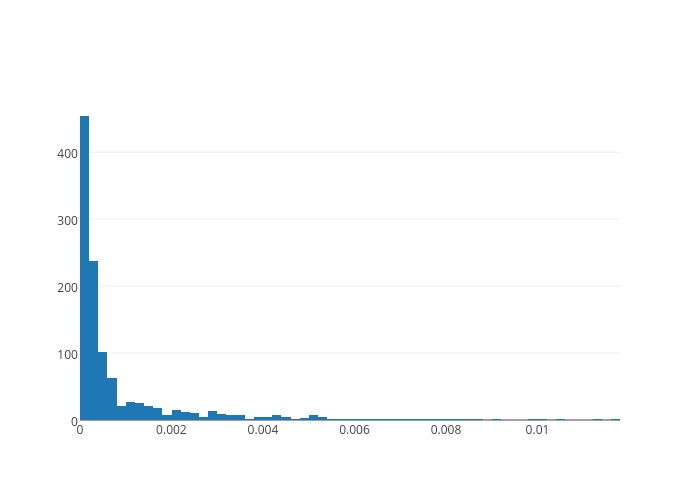
\includegraphics[width=0.28\textwidth]{0am-busy.jpeg}
\caption{Tuesday 12 am Workload Distribution}
\end{figure}
This is representative in all (day, hour) combinations. Apparently $p(\alpha, s)$ follows an exponential distribution, where
\begin{align}
p(\alpha, s) = \kappa\frac{L}{s}e^{-\kappa\frac{L}{s}\alpha}
\end{align}
Here $\frac{L}{s}$ is the scale factor for $\kappa$, where $L$ is the constant number of map size. This can be interpreted as the longer distance the driver traveled, the more he/she is likely to see the real distribution. With a small value of $s$ (short trip distance), by common sense, the driver is more likely to see grids with smaller $\omega$, equivalent to a steeper exponential probability curve after normalization. Now if I substitute $\kappa\frac{L}{s}$ as $\gamma$ into (5), I get 
\begin{align}
\int_{0}^{1}(1-\frac{1}{1+e^{-K(\omega-\mu_\omega)}})\gamma e^{-\gamma\omega}d\omega = \frac{1}{2}
\end{align}
For this equation to hold, I tune the steepness factor $K$ empirically as $\frac{\mu_\omega}{2\sigma_\omega^2}$. This setup is later proved to work out well.
With the cruise time calculated from $t_c = \frac{v_t}{\alpha v_g}$ and average waiting time $\lambda$, I sample from the process and calculate the pick-up probability:
\begin{align}
p &= \sum_{i=0}^{t_c}\frac{\lambda^ie^{-\lambda}}{i!}
\end{align}
\item Distribution mean, variance. I plot the histogram of trip distance, trip duration, and total pay amount starting from several POI's at different time on Tuesday in figure 2-4.
\begin{figure}
\centering
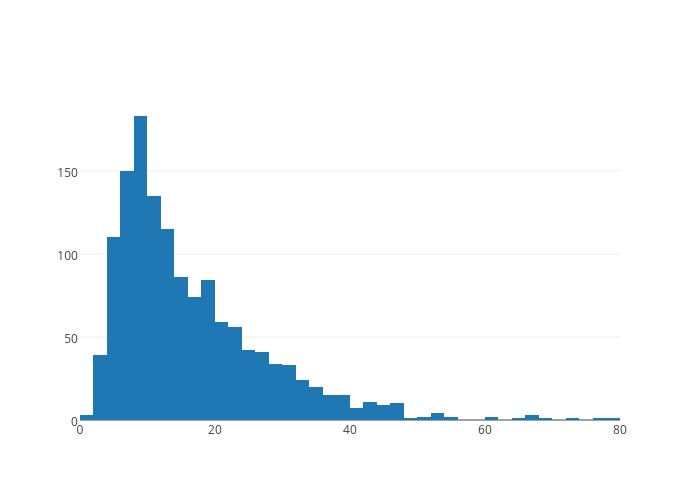
\includegraphics[width=0.28\textwidth]{5pm-littleitaly-soho-triptime.jpeg}
\caption{5 pm Little Italy SOHO Trip Time Distribution}
\end{figure}
\begin{figure}
\centering
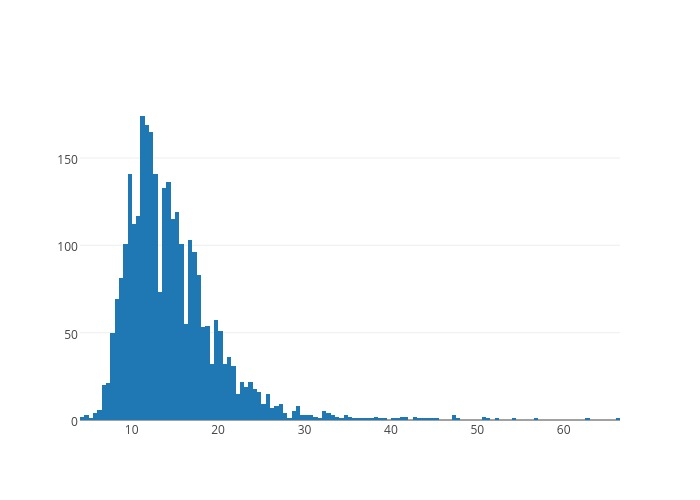
\includegraphics[width=0.28\textwidth]{18-lincoln-tunnel-pay.jpeg}
\caption{6 pm Lincoln Tunnel Pay Distribution}
\end{figure}
\begin{figure}
\centering
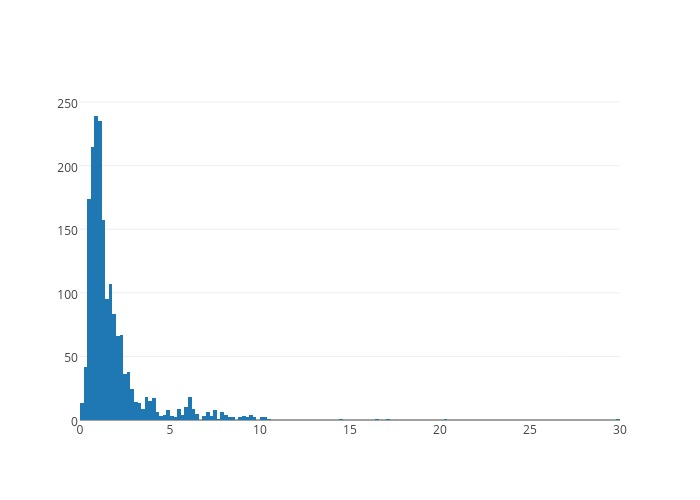
\includegraphics[width=0.28\textwidth]{11am-sutton-place-dist.jpeg}
\caption{11 am Sutton Place Trip Distance Distribution}
\end{figure}
Apparently, from the figures, I notice all three distributions are skewed normal. The means and variances of theses distributions are thus effective in evaluating the reward of a grid. Given the numbers, for the specific week day, I define the following reward function for a (grid, hour) key:
\begin{align}
R(g, t) = p\frac{(\mu_p-\frac{\sigma_p}{2})^2}{(\mu_t-\frac{\sigma_t}{2})(\mu_s-\frac{\sigma_s}{2})}
\end{align}
I will discuss later their usage in path simulation. 
\item Drop-off location probability map. This is crucial data for the MDP process and path simulation. Given location-time pair $(g, t)$, I store the mapping 
\begin{align}
\mathcal{M}:(g,t,g')\to \{\rho_{g'}\}
\end{align}
for all $g'$ in the drop-off location set $\mathcal{D}_{(g,t)}$, where $\rho$ is the probability of drop-off at $g'$. Note that $\sum_{g'}\rho_{g'}=1$.
\end{enumerate}
With above parameters described, I visualize a few pick-up probability maps of NYC, generated from a 15-month dataset. I also plot the drop-off location map from certain pick-up locations. See figure 5-9.
\begin{figure}
\centering
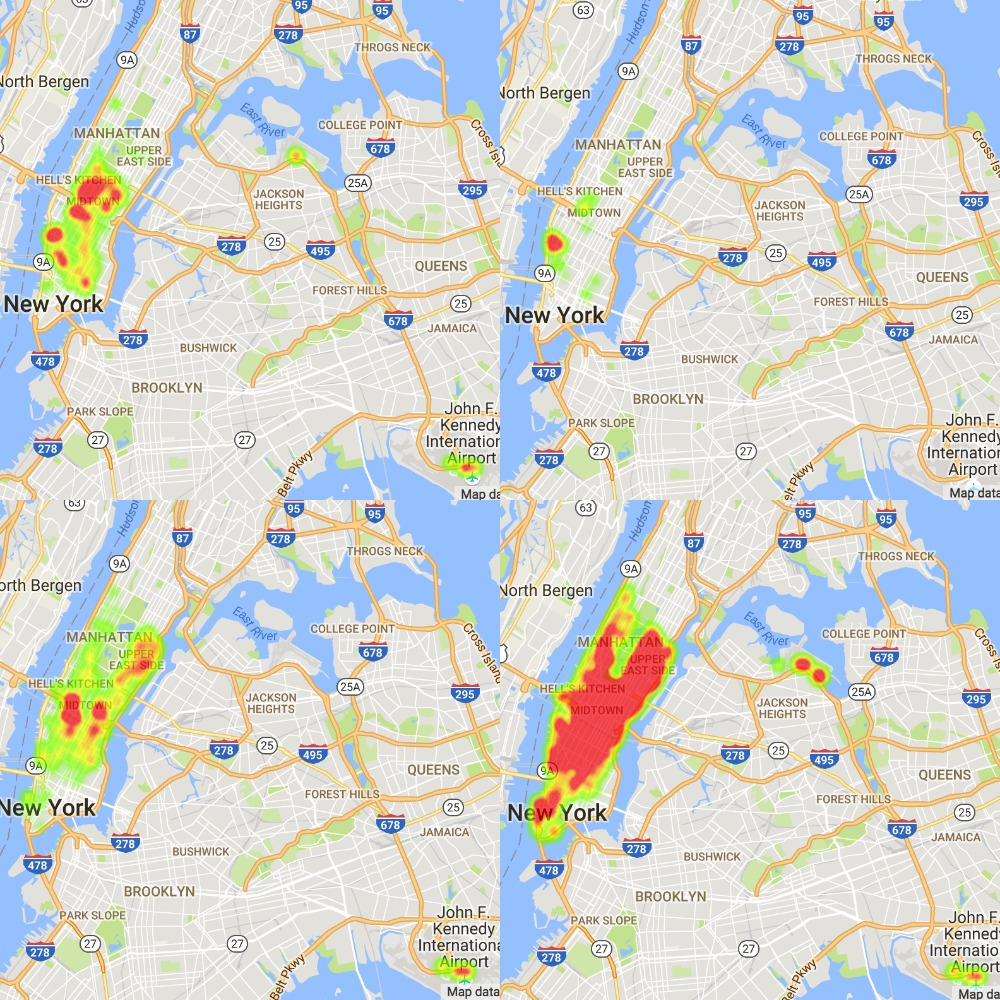
\includegraphics[width=0.3\textwidth]{0-9.jpg}
\caption{From Top-Left to Bottom-Right: 12 am, 3 am, 6 am, 9 am}
\end{figure}
\begin{figure}
\centering
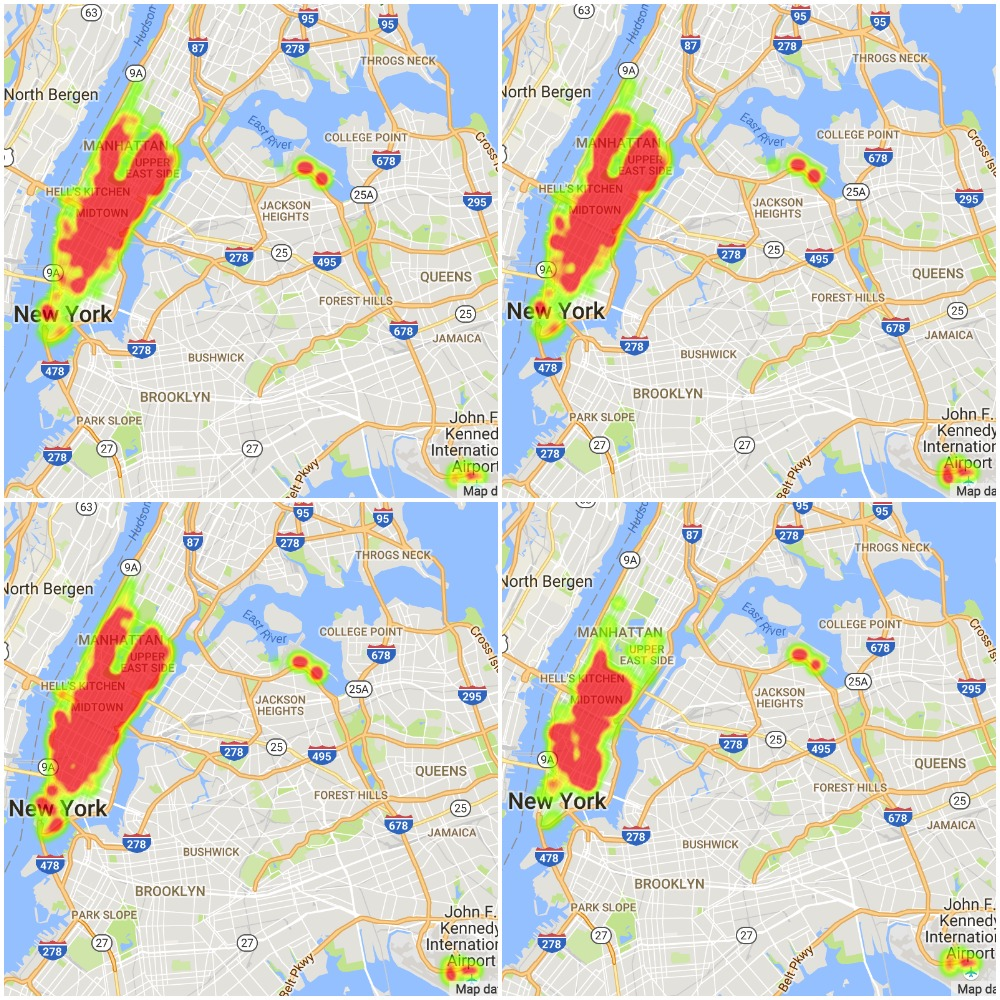
\includegraphics[width=0.3\textwidth]{12-23.jpg}
\caption{From Top-Left to Bottom-Right: 12 pm, 3 pm, 6 pm, 11 pm}
\end{figure}
\begin{figure}
\centering
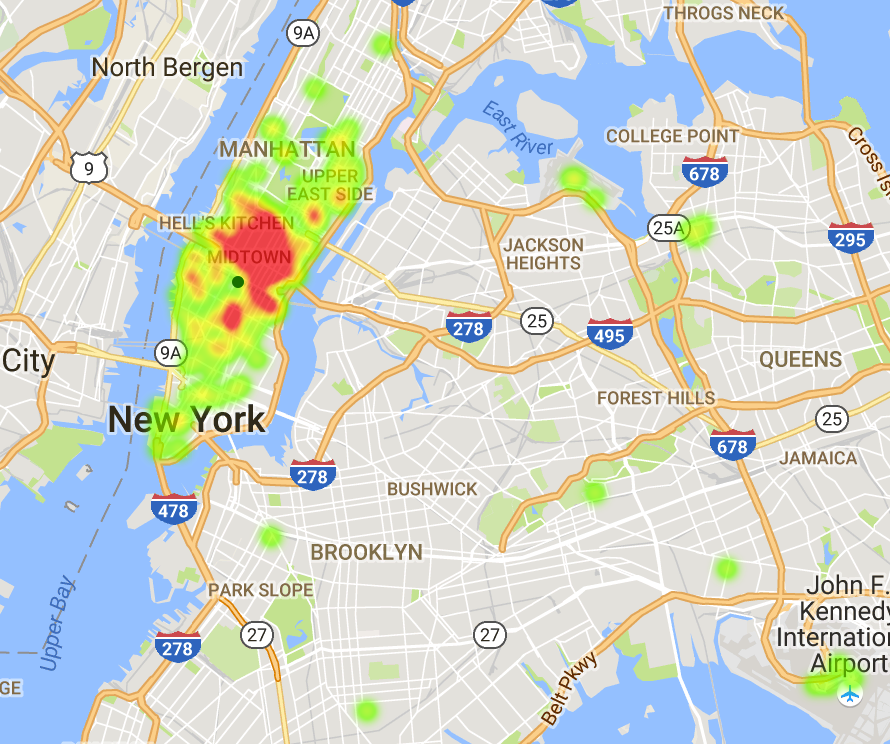
\includegraphics[width=0.33\textwidth]{5pm-empire-state.png}
\caption{5 pm Drop-off From Empire State Building}
\end{figure}
\begin{figure}
\centering
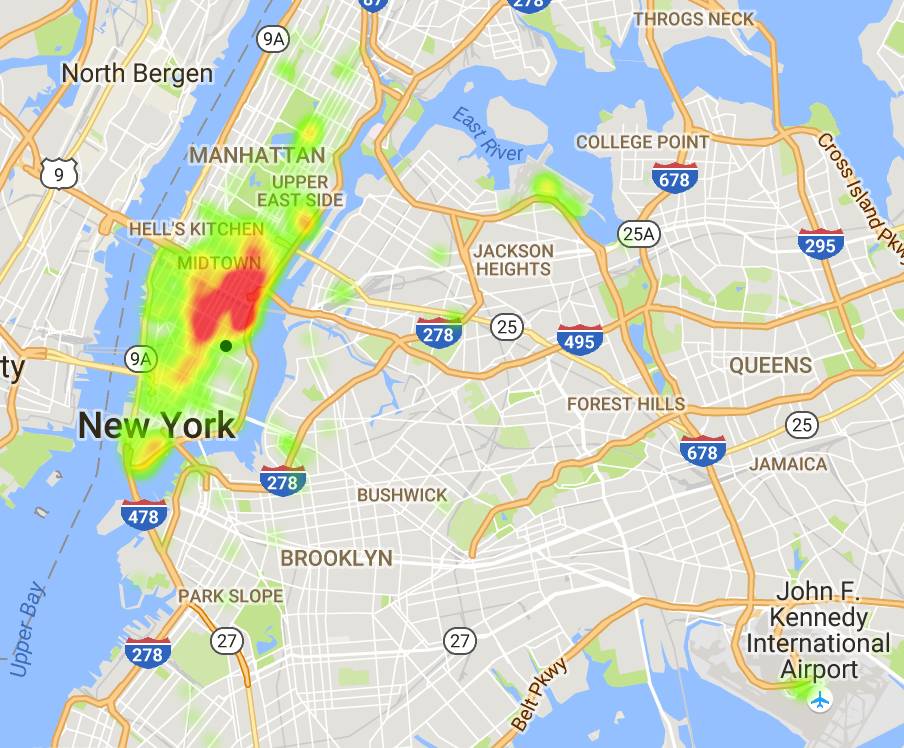
\includegraphics[width=0.33\textwidth]{9-MtSinaiHospital.png}
\caption{9 pm Drop-off From Mt. Sinai Hospital}
\end{figure}
\begin{figure}
\centering
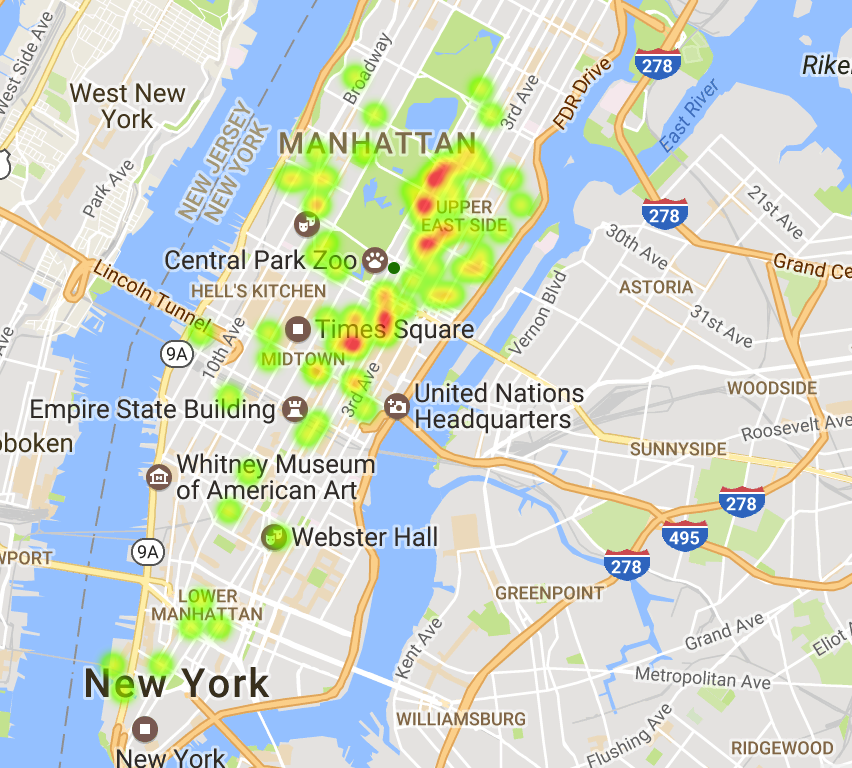
\includegraphics[width=0.33\textwidth]{11-chanel-shop.png}
\caption{11am Drop-off From Chanel Shop}
\end{figure}
\subsection{Markov Decision Process}
Now I formally define the MDP for the passenger pick-up problem.\\
\textbf{States}: $\mathcal{S} = \{(g, t): g\in\mathcal{B}\wedge t\in(T_s, T_e)\}$, where $T_s, T_e$ are start and end time (driver shift).\\
\textbf{s$_{\text{start}}$}$=(g_s, T_s)$ where $g_s$ is starting location.\\
\textbf{Actions$((g, t))$} =
\begin{align}
\{(g', t'):t'= t+t_s\wedge g'\in\mathcal{N}(g)\cup\mathcal{H}\}
\end{align}
where $t_s$ is the trip duration, $\mathcal{N}(g)$ is the neighbors of $g$ (including itself), and $\mathcal{H}$ is the set of hotspots on the map.\\
\textbf{Transition$((g,t), a, (g',t'))$}=
\begin{align}
1\{g'\in\mathcal{N}(g)\}(1-p_g)\\
+1\{g'\not\in\mathcal{N}(g)\}p_g\cdot\mathcal{M}_{(g,t,g')}
\end{align}
which can be viewed as two parts: if the taxi does not pick up a passenger in current location, then it can arrive in the neighbors; otherwise it can only arrive at location $g'$ if the passenger also goes there.\\
\textbf{Reward}$((g,t), a, (g',t'))=\frac{R(g,t)}{t'-t}$\\
This is simply dividing reward function (9) by the travel time towards $g'$. In current implementation $\delta_t$ is calculated by $\frac{g'-g}{v}+t_c$. The result can be more accurate by applying Bresenham's Algorithm, which is discussed in section VI.\\
\textbf{IsEnd}$((g,t))=1\{t>T_e\}$. Exceeds time limit.\\
\textbf{$\gamma$} = 1.


Now the logic behind the scene. There are many assumptions to make to solve the problem: if I assume the driver to pick up whenever he/she sees passengers on the way, then I can only allow Actions$((g,t))$ to be $\mathcal{N}$, otherwise there is no guarantee that the driver will ever arrive at any chosen $g'$. However, if I only allow Actions$((g,t))$ to be $\mathcal{N}$, then if the driver is in the middle of nowhere (unseen states in dataset), then he/she will get bogged. 

On the other hand, if I assume the driver only goes to chosen target $g'$ without taking any passengers midway, then I can allow Actions$((g,t))$ to be arbitrary $g'\in\mathcal{B}$. This setting explores the entire map with every possible situation, which finds the global optimum of the problem. However, this is computationally unacceptable. Instead, I decide to take a step back, and choose to search for local optimum: let Action$((g,t))$ to be $\mathcal{N}\cup\mathcal{H}$, a combination of neighbors and hotspots. This prevents the driver from wandering in nowhere and also stops him/her from over-exploiting the hotspots. This is an analogy of the Exploration-Exploitation problem, where $\epsilon$ stands for the size of $\mathcal{H}$. My assumption of not picking up midway also works perfectly here: if the driver is heading to the hotspots, the $g$'s on the path will not likely have high pick-up probabilities, otherwise, they are hotspots themselves.
\subsection{Policy Generation}
\subsubsection{Learned Policy}
I use value iteration method to generate the learned policy for MDP states. For each state $s$, compute the utility value as 
\begin{align}
U_{\text{opt}}^{(t)}\to \operatornamewithlimits{max}_{a\in \text{Actions}(s)}\sum_{s'}T(s,a,s')[R(s,a,s')+U_{\text{opt}}^{(t-1)}(s')]
\end{align}
Different from what I stated in the formulation of MDP above, in the actual implementation I choose states as the set of states appeared in dataset keys. This is to reduce unnecessary computation and expedite the iteration. If the successor $(g',t')$ from $(g,t)$ is unseen (new $t'$ from time elapse, or new $g'$ from wandering into neighbors), then I assume average $t_c$, $v$, and $p=0.0$, since not recorded means there is no previous pick-up event. The probability sums to 1 as follows:
\begin{align}
p + (1-p)\sum_{g'}\rho_{g'} =1
\end{align}
Figure 10 is the learning curve for value iteration.
\begin{figure}
\centering
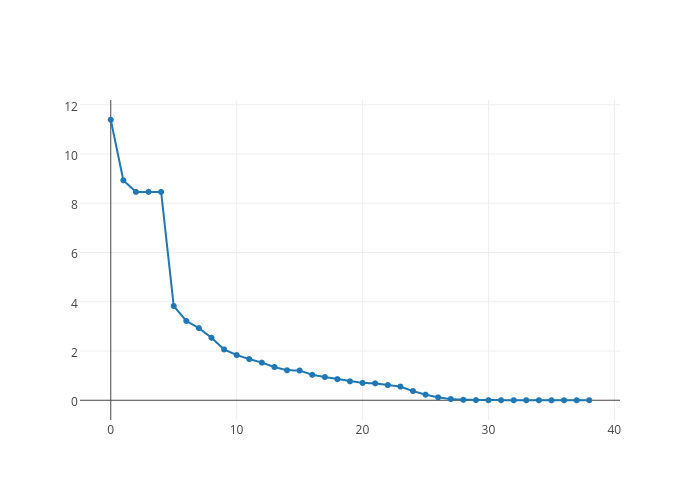
\includegraphics[width=0.33\textwidth]{tiny_VI_curve.png}
\caption{Value Iteration Learning Curve}
\end{figure}
\subsubsection{Baseline Policy}
An obvious baseline policy is to run randomly on $\mathcal{N}$. One disadvantage mentioned before is that the driver may run into unreachable spaces such as the middle of Central Park, or Hudson Bay. Using coordinates of POI's can solve this problem.
\subsubsection{Oracle Policy}
The main obstacle for achieving an oracle policy is that the TLC dataset is highly anonymous, with all license and Medallion ID erased from records, thus I cannot follow on individual taxis to directly pick out the route with maximum net profit. I come up with a dynamic programming get-around. Different from the baseline and learned policies, the oracle takes in the initial location $g_i$ to generate an optimal route. I first process the original data RDD to reverse link all states, so that a key-value pair has form of $s'\to(s,m(s,s'))$, where $m(s,s')$ is the utility earned by going from $s=(g,t)$ to $s'=(g',t')$, evaluated by the Reward function. The base case is initializing all utilities to be zero: $u_s=0$ for all $s\in\mathcal{S}$. Next, I define the transition function
\begin{align}
u_s &= \text{max}(u_{s'}+m(s, s'), m(s_i, s))
\end{align}
where $s_i$ is the initial state. Note that all unseen states are assigned with $u=0$. Backtracking the utility map, I get the oracle policy.
\section{Results}
\subsection{Policy Analysis}
I run the framework on the same small representative dataset, run generated policies on same location and time settings for 30 iterations, and use the average reward to evaluate the correctness of my methods. Below is the table comparing results from three policies.
\begin{center}
\begin{tabular}{|c||c|c|c|}
\hline
Policy & Profit & Depreciation & Performance \\ \hline
Baseline & 51.93 & 14.94 & 3.48 \\    \hline
Learned & 74.99 & 19.55 & 3.84 \\    \hline
Oracle & 79.97 & 20.66 & 3.87 \\    \hline
\end{tabular}
\end{center}
\subsection{Visualization of Simulated Path}
In order to better extrapolate the feasibility and correctness of my framework, I run the generated policies on my simulator and visualize some representative routes in figure 11-13, starting from Tuesday 12:01 AM from Empire State Building, driving for 80 minutes. The full visualization part is included in the code repository, with drop pins marking earned money, and time. In simulation phase, I sample the multinomial drop-off locations from $\mathcal{M}$. Note that the profit values are higher than the actual case of average 50\$, due to the slightly large fare rate in the simulation.
\begin{figure}
\centering
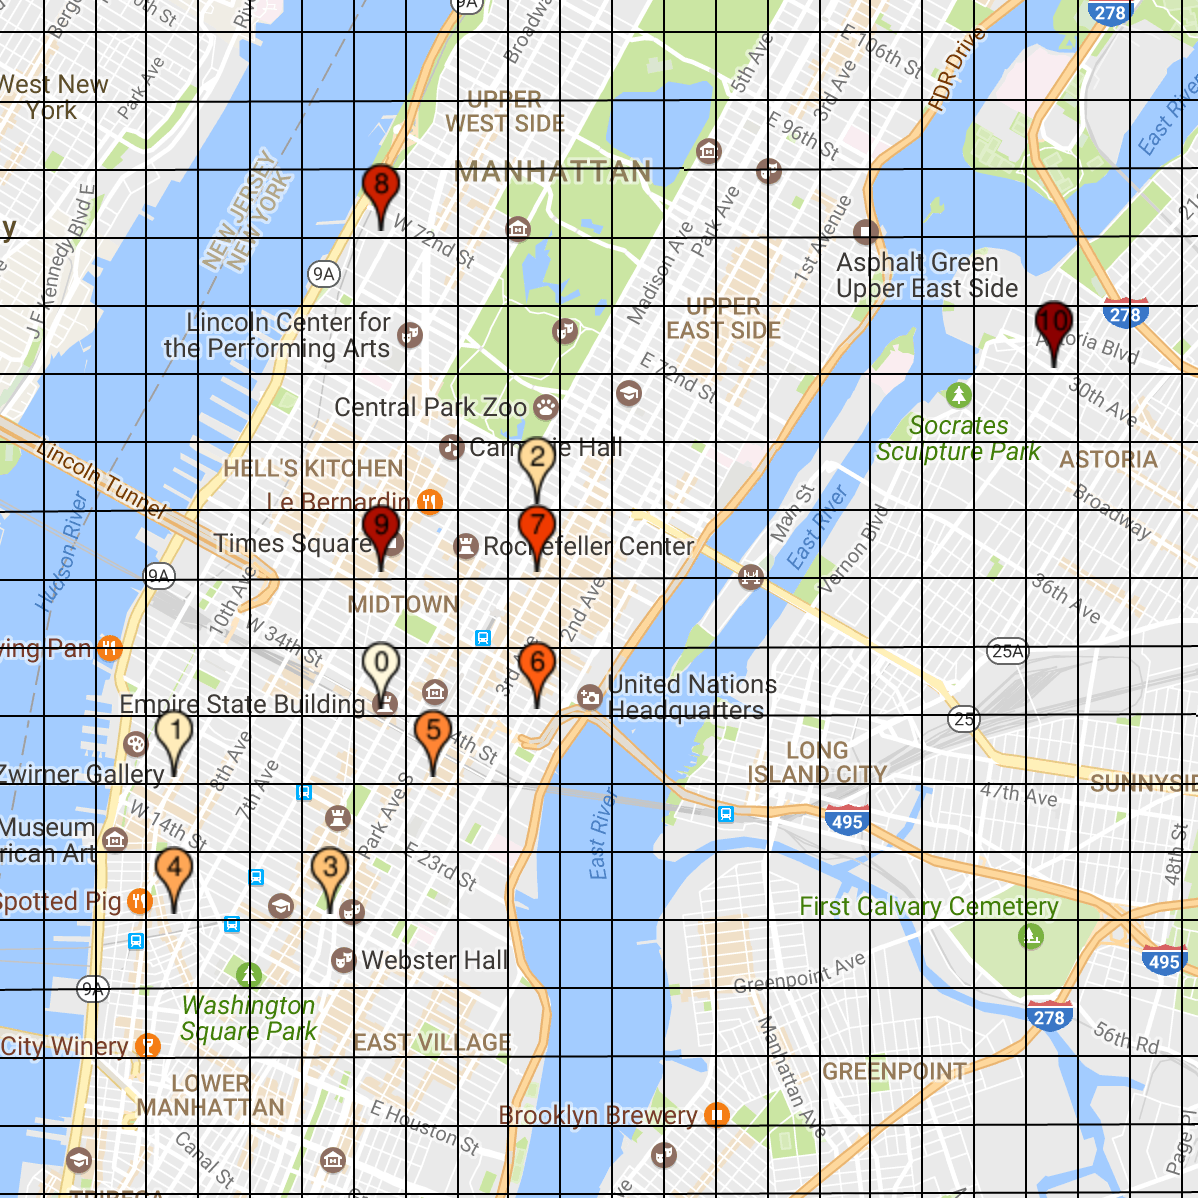
\includegraphics[width=0.3\textwidth]{oracle.png}
\caption{Oracle Route. Earned 104.01\$}
\end{figure}
\begin{figure}
\centering
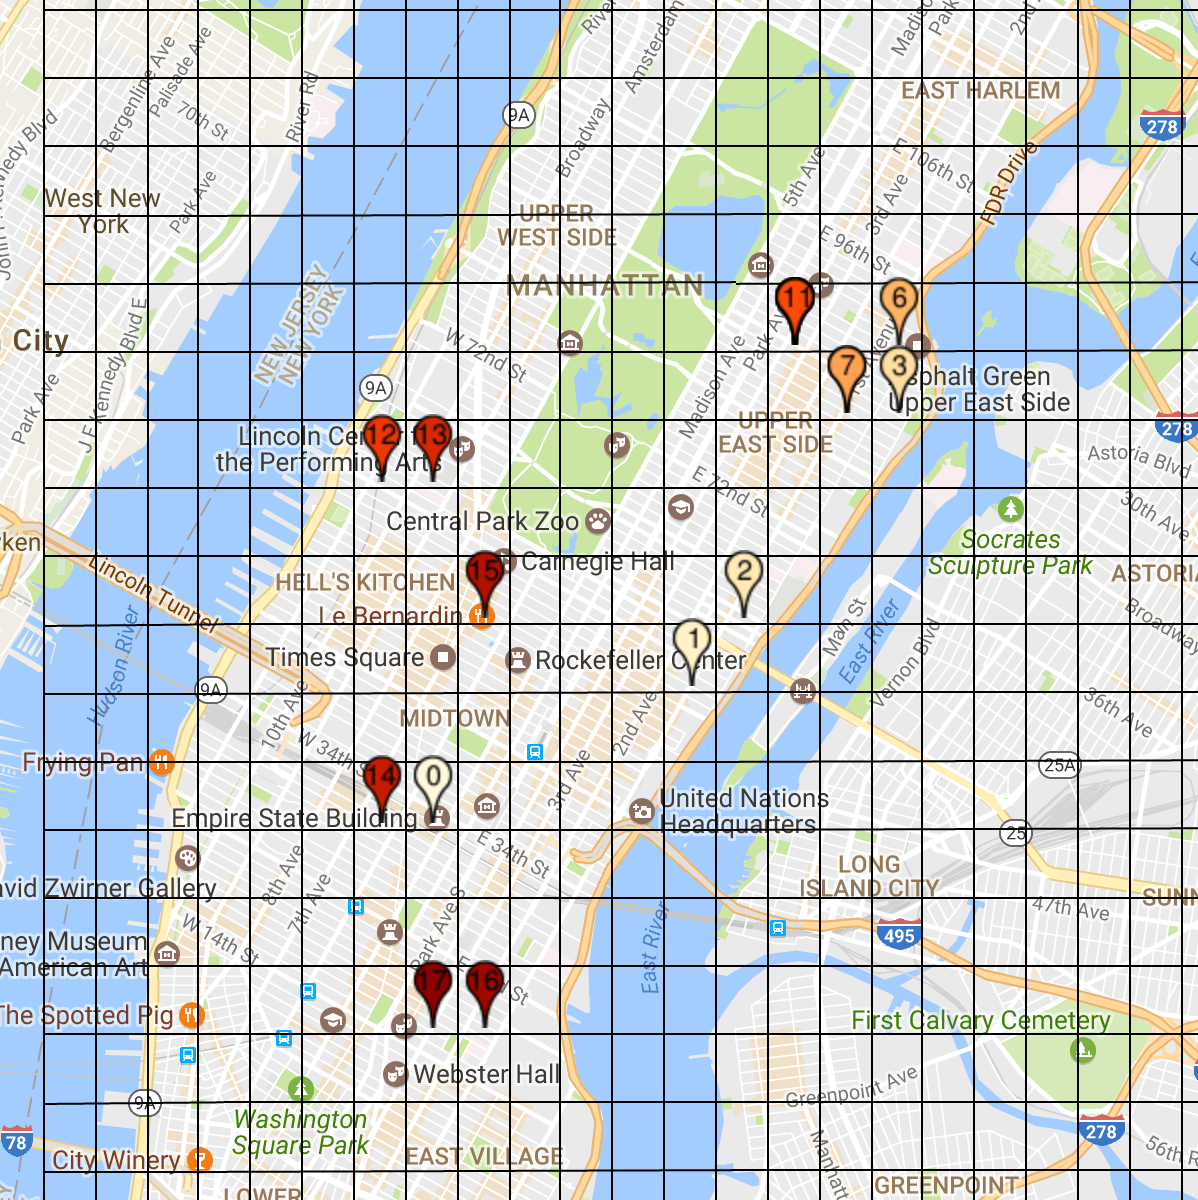
\includegraphics[width=0.3\textwidth]{learned.png}
\caption{Learned Route. Earned 83.80\$}
\end{figure}
\begin{figure}
\centering
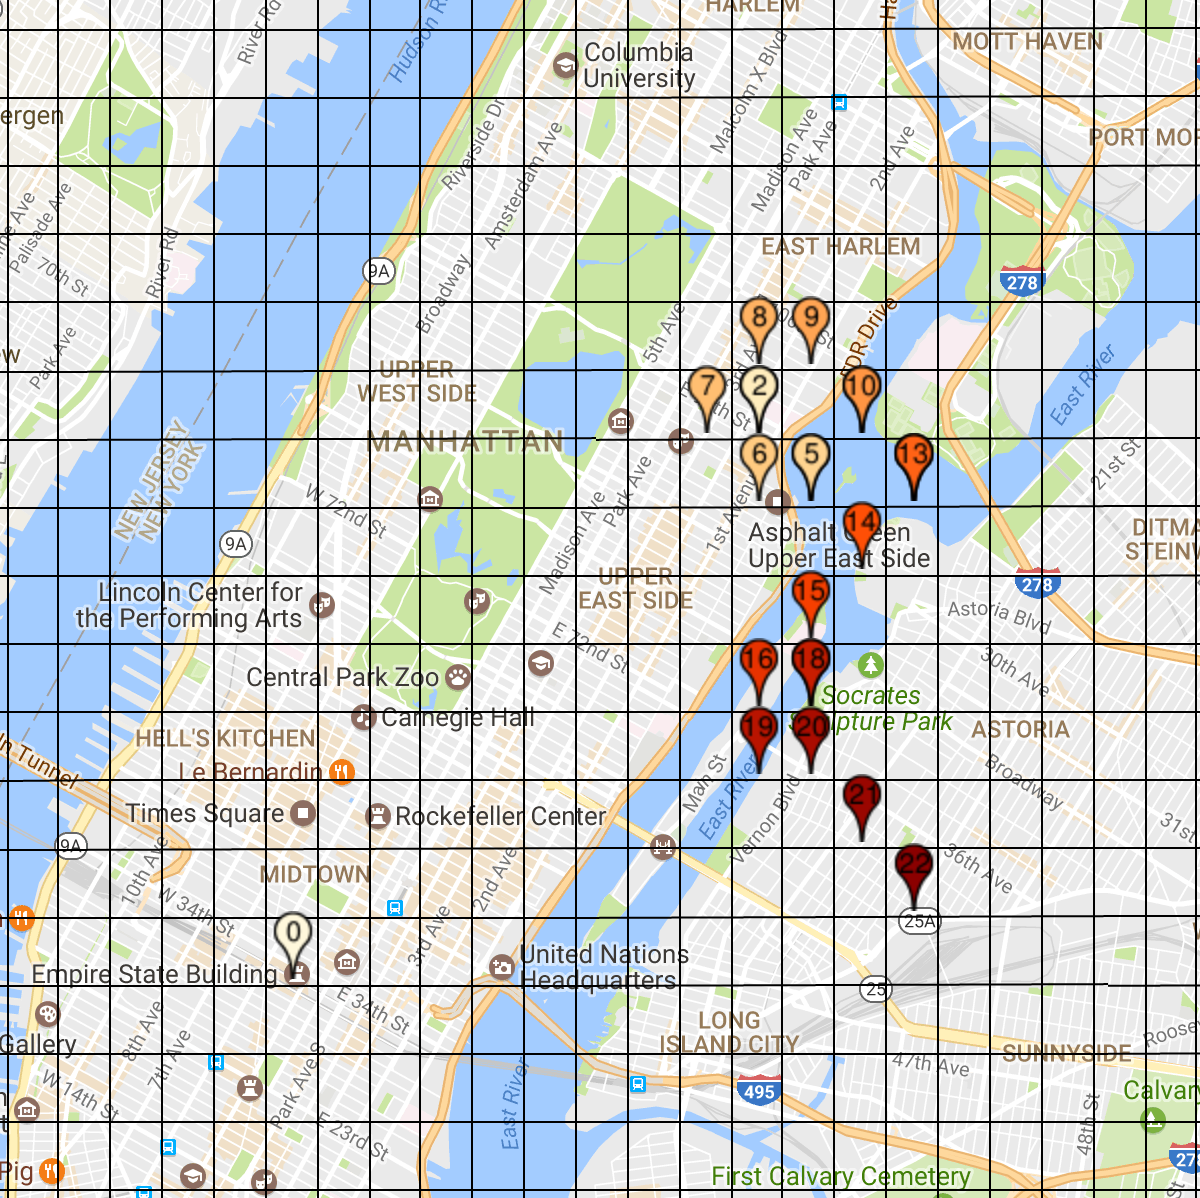
\includegraphics[width=0.3\textwidth]{baseline.png}
\caption{Baseline Route. Earned 25.09\$}
\end{figure}
\section{Future Works}
As mentioned previously, the gridify process is a bold assumption I make, and migrate to POI GPS coordinates can make the framework more accurate. In evaluating travel time from current location to target location, I simply divide the straight line distance by the average speed, which is not ideal. The Bresenham's Algorithm determines the points of an n-dimensional raster that should be selected in order to form a close approximation to a straight line between two points\cite{bresenham}, from where I can make use of congestion factors along the path and get a more accurate estimation of travel time between grids. As a side mark, I will run on larger dataset for more comprehensive policies, with extra computational resources such as AWS. Code available on GitHub repository:
\begin{center}
\textit{https://github.com/JulianYG/221finalproject}
\end{center}
\bibliographystyle{ieeetr}
\bibliography{report}
\end{document}
